
\section{Configuración experimental}

La configuración experimental sigue un enfoque supervisado. En la cual se cuenta con un conjunto de historiales de usuario, los cuales pueden verse como un sólo documento, a este documento $X$ le corresponde su etiqueta correspondiente $y \in Y$  en una relación uno a uno. En todos los conjuntos de datos usados se trata únicamente de dos clases, es decir, se trata de una clasificación binaria ($|Y| = 2$). 

La metodología empleada está compuesta de 4 fases:  preprocesamiento, aumento de datos, entrenamiento y evaluación. En el preprocesamiento, se realizan las modificaciones necesarias para normalizar los documentos, además de segmentarlos y filtrarlos en secuencias de 64 palabras, este valor fue encontrado empíricamente para optimizar el aprendizaje en las redes neuronales; posteriormente, continúa la etapa de aumento de datos. Una vez que se han aumentado los datos de entrenamiento para la clase de interés, se construye un modelo de clasificación, mediante un algoritmo de aprendizaje automático (en específico, es de nuestro interés los métodos de redes profundas). Finalmente, se evalúa el modelo de clasificación sobre un conjunto de datos que no ha sido aumentado ni utilizado en la búsqueda de parámetros durante el entrenamiento, únicamente es preprocesado de la misma forma que los datos de entrenamiento. La figura \ref{fig:metodologia} muestra las diferentes fases descritas. 

\begin{figure}[h]
    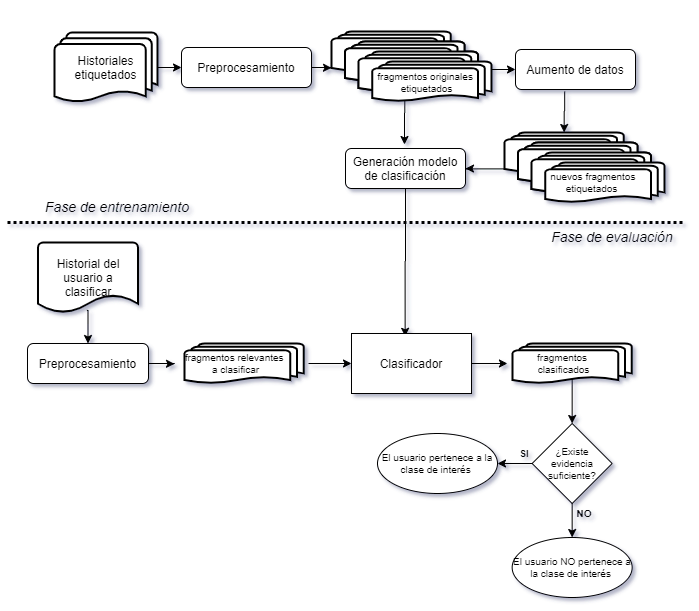
\includegraphics[width=\textwidth]{sections/figures/diagrama_general.png}
    \caption{Diagrama general de la configuración experimental}
    \label{fig:metodologia}
\end{figure}

\subsection{Conjunto de datos}

\textbf{Depresión 2018 y Anorexia}: Con el propósito de estudiar la detección temprana de depresión y anorexia, los autores \citep{Losada2018} recopilaron publicaciones de usuarios diversos, de la red social Reddit. Para cada usuario la colección contiene una secuencia de publicaciones en orden cronológico. Este conjunto de datos, se caracteriza por tener una gran cantidad de texto, pero con muy pocos usuarios, como se puede observar en la figura \ref{fig:erisk_freq}. Hay dos categorías para cada usuario en cada tarea. El número de usuarios total en cada conjunto se presenta en la tabla \ref{table:original_users}. Dado que se trabaja con conjuntos de datos muy desbalanceados, el aumento de datos solo se aplica sobre la clase de interés o clase positiva.

\textbf{Depresión 2019}: Presentado en las tareas eRisk 2019 \cite{Losada2019}, a diferencia de la edición 2018, en esta ocasión el objetivo es predecir los niveles de depresión de un usuario (mínima, media, moderada, severa). Con el objetivo de que los resultados sean comparables, en este trabajo el problema fue reducido a una clasificación binaria, al igual que el conjunto de 2018; para esto los usuarios con depresión media a severa se tomaron como ejemplos de la clase positiva.

Para el entrenamiento solo se consideraron 16 usuarios para la clase positiva como se muestra en la tabla \ref{table:original_users}, para obtener usuarios de la clase negativa, se tomaron los usuarios etiquetados como no deprimidos del conjunto de entrenamiento eRisk 2018. Finalmente, el conjunto de evaluación, solo se dividió en dos clases quedando 60 positivos y 10 negativos (deprimidos y no deprimidos respectivamente).
\begin{table}[!hbt]
\caption{Número de usuarios en los conjuntos de datos y número de sub-documentos con 64 palabras después del pre-procesamiento, sin aplicar el filtro de sub-documentos.} \label{table:orginal_users}
\begin{center}

\begin{tabular}{llll}
\hline
\rowcolor[HTML]{FFFFFF} 
\textbf{Usuarios}                                           & \textbf{Entrenamiento}                       & \textbf{Evaluación}                          & \textbf{Vocabulario}                                         \\ \hline
\rowcolor[HTML]{EFEFEF} 
\textit{Conjunto 1: Depresión 2018}                         & \multicolumn{1}{c}{\cellcolor[HTML]{EFEFEF}} & \multicolumn{1}{c}{\cellcolor[HTML]{EFEFEF}} &                                                              \\ \hline
\rowcolor[HTML]{FFFFFF} 
deprimido                                                   & 135 - 31,396                                 & 79 - 25,967                                  &                                                              \\ \hline
\rowcolor[HTML]{FFFFFF} 
no-deprimido                                                & 752 - 227,189                                & 741 - 272,703                                &                                                              \\ \hline
\rowcolor[HTML]{FFFFFF} 
\textbf{Total}                                              & \textit{887 - 138,232}                       & \textit{820 - 298,670}                       & \multicolumn{1}{c}{\cellcolor[HTML]{FFFFFF}\textit{202,151}} \\ \hline
\rowcolor[HTML]{EFEFEF} 
\cellcolor[HTML]{EFEFEF}\textit{Conjunto 2: Depresión 2019} &                                              &                                              &                                                              \\ \hline
\rowcolor[HTML]{FFFFFF} 
deprimido                                                   & 16 - 5,731                                   & 60 - 18,534                                  &                                                              \\ \hline
\rowcolor[HTML]{FFFFFF} 
no-deprimido                                                & 752 - 227,189                                & 10 - 5,011                                   &                                                              \\ \hline
\rowcolor[HTML]{FFFFFF} 
\textbf{Total}                                              & \textit{768 - 232,920}                       & \textit{70 - 23,545}                         & \multicolumn{1}{c}{\cellcolor[HTML]{FFFFFF}\textit{195,047}}    \\ \hline
\rowcolor[HTML]{EFEFEF} 
\textit{Conjunto 3: Anorexia}                               & \multicolumn{1}{c}{\cellcolor[HTML]{EFEFEF}} & \multicolumn{1}{c}{\cellcolor[HTML]{EFEFEF}} &                                                              \\ \hline
\rowcolor[HTML]{FFFFFF} 
con anorexia                                                & 61 - 23,335                                  & 73 - 16,751                                  &                                                              \\ \hline
\rowcolor[HTML]{FFFFFF} 
sin-anorexia                                                & 411 - 36,484                                 & 742 - 254,640                                &                                                              \\ \hline
\rowcolor[HTML]{FFFFFF} 
\textbf{Total}                                              & \textit{472 - 130,574}                       & \textit{815 - 271,391}                       & \multicolumn{1}{c}{\cellcolor[HTML]{FFFFFF}\textit{67,724}}  \\ \hline
\end{tabular}

\end{center}

\end{table}


\begin{table}[!hbt]
\caption{Número de usuarios en los conjuntos de datos y número de secuencias con 64 palabras después del pre-procesamiento, realizando el filtro. Los números resaltados en negritas representan el numero de historiales comparado con el numero de secuencias} \label{table:filter_users}

\resizebox{\textwidth}{!}{%

\begin{tabular}{llll}
\hline
\rowcolor[HTML]{FFFFFF} 
\textbf{Usuarios}                   & \textbf{Entrenamiento}                       & \textbf{Evaluación}                          & \textbf{Vocabulario}                                         \\ \hline
\rowcolor[HTML]{EFEFEF} 
\textit{Conjunto 1: Depresión 2018} & \multicolumn{1}{c}{\cellcolor[HTML]{EFEFEF}} & \multicolumn{1}{c}{\cellcolor[HTML]{EFEFEF}} &                                                              \\ \hline
\rowcolor[HTML]{FFFFFF} 
deprimido                           & \textbf{135} - 24,483                                 & \textbf{79} - 25,967                                  &                                                              \\ \hline
\rowcolor[HTML]{FFFFFF} 
no-deprimido                        & \textbf{744} - 98,783                                 & \textbf{741} - 272,703                                &                                                              \\ \hline
\rowcolor[HTML]{FFFFFF} 
\textbf{Total}                      & \textit{\textbf{879} - 123,266}                       & \textit{\textbf{820} - 298,670}                       & \multicolumn{1}{c}{\cellcolor[HTML]{FFFFFF}\textit{104,800}} \\ \hline
\rowcolor[HTML]{EFEFEF} 
\textit{Conjunto 2: Depresión 2019} & \multicolumn{1}{c}{\cellcolor[HTML]{EFEFEF}} & \multicolumn{1}{c}{\cellcolor[HTML]{EFEFEF}} &                                                              \\ \hline
\rowcolor[HTML]{FFFFFF} 
deprimido                           & \textbf{16} - 5,731                                   & \textbf{60} - 18,534                                  &                                                              \\ \hline
\rowcolor[HTML]{FFFFFF} 
no-deprimido                        & \textbf{746} - 125,823                                & \textbf{10} - 5,011                                   &                                                              \\ \hline
\rowcolor[HTML]{FFFFFF} 
\textbf{Total}                      & \textit{\textbf{762} - 131,554}                       & \textit{\textbf{70} - 23,545}                         & \multicolumn{1}{c}{\cellcolor[HTML]{FFFFFF}\textit{118,668}}    \\ \hline
\rowcolor[HTML]{EFEFEF} 
\textit{Conjunto 2: Anorexia}       & \multicolumn{1}{c}{\cellcolor[HTML]{EFEFEF}} & \multicolumn{1}{c}{\cellcolor[HTML]{EFEFEF}} &                                                              \\ \hline
\rowcolor[HTML]{FFFFFF} 
con anorexia                        & \textbf{61}-23,335                                    & \textbf{73}-16,751                                    &                                                              \\ \hline
\rowcolor[HTML]{FFFFFF} 
sin-anorexia                        & \textbf{411}-107,239                                  & \textbf{742}-254,640                                  &                                                              \\ \hline
\rowcolor[HTML]{FFFFFF} 
\textbf{Total}                      & \textit{\textbf{472}-130,574}                         & \textit{\textbf{815}-271,391}                         & \multicolumn{1}{c}{\cellcolor[HTML]{FFFFFF}\textit{131,264}} \\ \hline
\end{tabular}

}

\end{table}



%[!htbp]
\begin{figure}[!ht]
    
    \begin{subfigure}[b]{0.5\textwidth}
        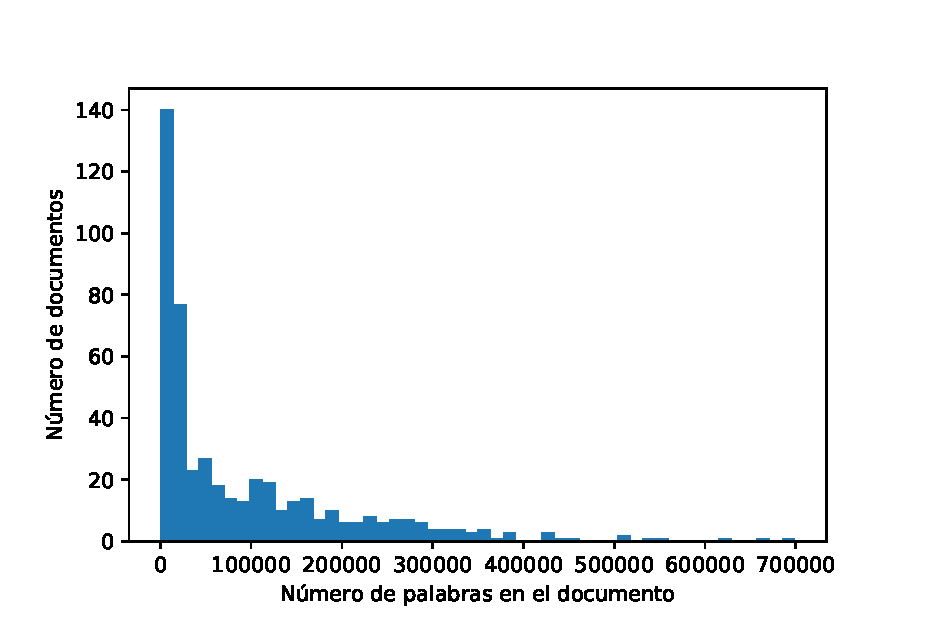
\includegraphics[width=\textwidth]{sections/figures/length_dist.eps}
        \caption{Depresión}
    \end{subfigure}
    \hfill
    \begin{subfigure}[b]{0.5\textwidth}
        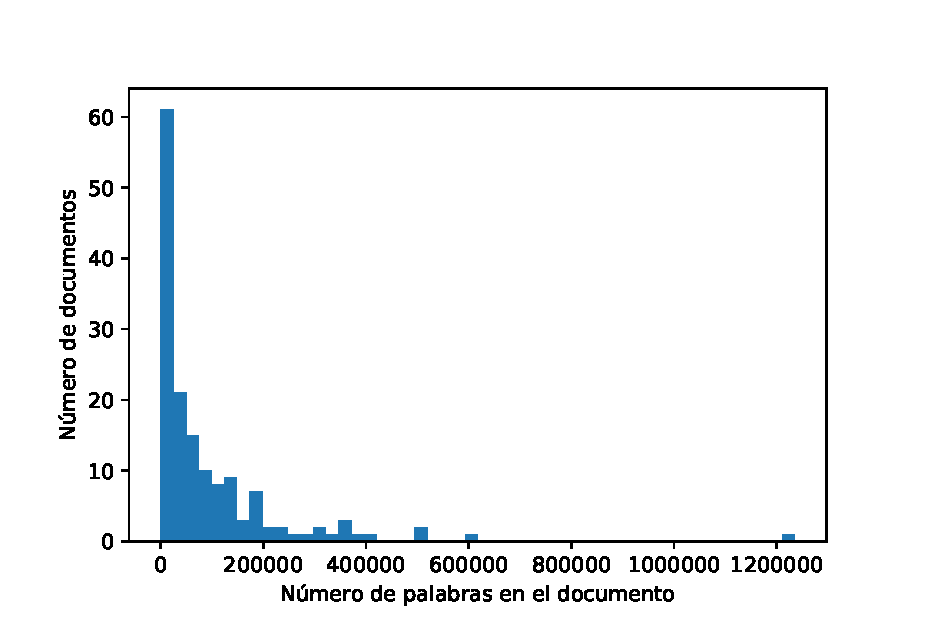
\includegraphics[width=\textwidth]{sections/figures/length_dist_anorexia.eps}
        \caption{Anorexia}
    \end{subfigure}
    \caption{Distribución del numero de palabras en los conjuntos de datos estudiados}
    \label{fig:erisk_freq}
\end{figure}

%% Agregar las distribución del conjunto anorexia


\subsection{Preprocesamiento}

Dado que los documentos extraídos de redes sociales no siguen un lenguaje formal y además de texto, existen direcciones de páginas web que los usuarios comparten, emoticonos y caracteres especiales, entre otros; es necesario que antes del aumento de datos exista un preprocesamiento de los textos como una forma de reducir el ruido de los documentos originales.

Los pasos del procesamiento seguido, son los siguientes:

 \begin{enumerate}
     \item Normalización: Se identifican las páginas web en el texto y se reemplazan mediante la etiqueta \textit{http}.
     \item Tokenización: Utilizando la herramienta NLTK se remueve de cada texto signos de puntuación y caracteres especiales.
     \item Segmentación: Los documentos originales son segmentados en pequeños fragmentos. Es decir, cada historial de usuario se fragmenta en secuencias de 64 palabras  (véase la siguiente sección).
     \item Filtrado: Solo se conservan segmentos identificados como importantes para la clasificación (véase la siguiente sección).
 \end{enumerate}



\subsubsection{Segmentación y filtrado}
Con el propósito de que el aumento de datos pueda ser proporcional independientemente de la longitud del documento original, cada documento se dividió en segmentos de 64 palabras\footnote{Este parámetro se determinó de manera empírica.}. Posteriormente, se filtró el conjunto de entrenamiento para conservar solo los segmentos importantes para realizar la clasificación. Es decir, se identificaron aquellos fragmentos con la mayor cantidad de palabras discriminantes. Para esto se identificaron las palabras más discriminantes dentro del vocabulario del conjunto de entrenamiento, mediante la técnica de selección de características $\chi^2$. Posteriormente, se conservaron aquellos fragmentos  que contengan un número determinado de palabras con alta puntuación $\chi^2$. 

Específicamente, solo se seleccionaron términos estadísticamente significativos al nivel 0.001, equivalente a una puntuación $\chi^2 > $ 10.83 con un grado de libertad. En la tabla \ref{table:filter_users} se muestran los números de usuarios y secuencias obtenidas después de aplicar este filtro; para el conjunto de depresión el criterio de selección fue que la secuencia contuviera al menos 20 palabras de 1071 palabras con alta puntuación, y para el conjunto de anorexia 18 palabras de 1032. Como puede observarse en ambos casos se trata de umbrales altos. Esto se debe principalmente a que en las palabras con alta puntuación se consideran palabras vacías, palabras que tradicionalmente se eliminan para tareas de clasificación temática. No obstante, en nuestro caso,  se trata de una tarea donde el estilo es importante (p.e. uso de pronombres personales).



\subsection{Configuración de los métodos propuestos}

Para comprobar la efectividad del método propuesto se experimenta con 7 configuraciones diferentes: 2 líneas base, 2 métodos del estado del arte y 3 métodos propuestos. Además de esto se introduce un parámetro $n$ para observar el grado pertinente del aumento de datos, el cual indica el número de documentos nuevos aumentados por cada documento original, tomando valores enteros en el rango $[1,10]$. Por lo tanto, para todos los métodos propuestos y de comparación (o referencia) solo se aumenta la clase positiva $n$ veces, desde $n=1$ hasta $n=10$.


\subsubsection{Sin aumento de datos}
Este método es la primera línea base y solo considera los datos originales filtrados para el entrenamiento de los modelos (véase la tabla \ref{table:filter_users}).

\subsubsection{Sobremuestreo}
Esta línea base, consiste en incrementar el número de ejemplos de la clase minoritaria mediante su replicación; este método no implica ninguna pérdida de información, ya que ningún elemento es modificado ni descartado. Sin embargo, la única desventaja es que el modelo de aprendizaje generado tiende a sobre ajustarse, debido a que no agrega variabilidad en los datos.

\subsubsection{Tesauro}
Este método del estado del arte fue propuesto por \citep{zhang2015character} y demostró mejoras de un 1 a un 2\% en exactitud para la clasificación de opiniones. También fue implementado por \citep{wei2019eda} con algunas modificaciones obteniendo una mejora entre un 1 y un 2\% en comparación de no hacer aumento de datos, otros trabajos que utilizan este método como referencia y han encontrado evidencia de que agrega una ganancia en los resultados de clasificación son: \citep{jungiewicz2019towards}, \citep{kumar2019submodular}, \citep{park2019self}.

Para decidir cuantas palabras reemplazar dada una secuencia de palabras, se calcula un número aleatorio $r$, generado de una distribución geométrica con un parámetro $p=$0.5; el recurso externo para encontrar sinónimos es un tesauro (en este caso Wordnet\footnote{www.wordnet.princeton.edu/}), y finalmente en la fase de reemplazo, de las palabras candidatas, se selecciona un número aleatorio $s$ generado de una distribución geométrica con parámetro $q=$ 0.5.

El propósito de este método es, ser muy conservativo en la modificación del texto original y el número $s$ controla la diversidad del vocabulario que por lo general para decidir qué palabras reemplazar empleada la palabra más utilizada.

\subsubsection{Sustitución sin restricción y reemplazo mediante similitud coseno}
Diversos estudios sugieren utilizar vectores de modelos preentrenados como Word2Vec, Glove, entre otros; la idea es recuperar palabras que se utilizan en contextos similares, en lugar de sinónimos. 

Para decidir qué palabras reemplazar se omiten palabras de paro y aquellas que no sean etiquetadas como sustantivos, adjetivos, verbos y adverbios; con el propósito de agregar más variabilidad en los ejemplos el número $r$ es calculado con el parámetro $p=$ 0.2. En la fase de reemplazo las palabras más similares se seleccionan mediante similitud coseno, utilizándolas de mayor a menor en una selección sin reemplazo.

El modelo de vectores preentrenados para representar las palabras de una secuencia fue Glove\footnote{https://nlp.stanford.edu/projects/glove/}, con 300 dimensiones \citep{pennington2014glove}. Este modelo fue preentrenado con la base de datos Common Crawl, con 42 millones de tokens y 1.9 millones de palabras. 


\subsubsection{Sustitución con restricción $\chi2$  y reemplazo mediante similitud relacional}
A diferencia del método anterior, una vez calculado el número $r$ de palabras a reemplazar, se omiten las palabras con mayor puntuación $\chi^2$ con un nivel de significación estadística de 0.001. 


\subsubsection{Reemplazo mediante similitud relacional equivalente}
En la fase de selección se fija el valor del parámetro $p=$ 0.2 y en la fase de reemplazo se utiliza la similitud relacional equivalente; esto es, obtener un vocabulario muy similar a la etiqueta de la clase, pero no el mismo. Las relaciones buscadas se listan en la tabla \ref{table:etiquetas}, para cada tarea de clasificación. Por ejemplo, para buscar las palabras candidatas a la palabra ``boyfriend", se utiliza la relación \textit{``depressed"} es a \textit{``boyfriend"} como \textit{``anxious"} es a \textbf{?}. 

\subsubsection{Reemplazo mediante similitud relacional contraria}
Este último método es similar al método anterior, lo único que cambia es la clase objetivo, en este caso se toman los documentos de clase opuesta (la clase negativa). Por ejemplo, para buscar las palabras candidatas a la palabra ``boyfriend", se utiliza la relación \textit{``happiness"} es a \textit{``boyfriend"} como \textit{``anxious"} es a \textbf{?}. La tabla \ref{table:etiquetas} resume las etiquetas empleadas para hacer el aumento.


\begin{table}[!hbt]
\caption{Etiquetas utilizadas en el proceso de aumento para los métodos de similitud relacional.} \label{table:etiquetas}
\begin{center}

\begin{tabular}{llll}
\hline
\rowcolor[HTML]{C0C0C0} 
Conjunto           & Clase & Etiqueta  & Palabra relacionada \\ \hline
\textbf{Depresión} & 1     & depressed & anxious           \\ \hline
                   & 0     & happiness & frustrated        \\ \hline
                   &       &           & unhappy           \\ \hline
                   &       &           & despondent        \\ \hline
                   &       &           & discouraged       \\ \hline
\textbf{Anorexia}  & 1     & anorexic  & bulimic           \\ \hline
                   & 0     & healthy   & underweight       \\ \hline
                   &       &           & obese             \\ \hline
                   &       &           & malnourished      \\ \hline
                   &       &           & unhealthy         \\ \hline
\end{tabular}

\end{center}
\end{table}


\subsubsection{Ejemplos del aumento de datos}
En la tabla \ref{table:ejemplos_pos} se presentan diversos ejemplos de aumento, el método basado en tesauro agrega un vocabulario más formal, en comparación con los basados en similitudes relacionales. El método basado en restricción $\chi^2$ conserva palabras importantes como ``feel", mientras que los demás no toman en consideración esto. Por otra parte, el método basado en relaciones equivalentes agrega la palabra \textit{``unfortunate"} como una palabra relacionada a la palabra \textit{``unhappy"}. 

\begin{table}[hbt!]
\caption{Ejemplos del aumento de datos.} 
\label{table:ejemplos_pos}
\begin{center}

\begin{tabular}{ll}
\hline
\rowcolor[HTML]{EFEFEF} 
\textbf{Método} & \textbf{Secuencia}                                                            \\ \hline
\rowcolor[HTML]{FFFFFF} 
Sin Aumento     & a lot of the time i have trouble communicating why i feel so unhappy          \\ \hline
\rowcolor[HTML]{FFFFFF} 
Thesauro        & a lot of the time i hold trouble communicating why i feel thusly infelicitous \\ \hline
\rowcolor[HTML]{FFFFFF} 
Sin Restricción & a lots of the time i have trouble communicating why i feeling so unhappy      \\ \hline
\rowcolor[HTML]{FFFFFF} 
Restricción Xi2 & a lot of the time i have difficulty informing why i feel so unhappy           \\ \hline
\rowcolor[HTML]{FFFFFF} 
Equivalencia    & a much of the place i have troubles informing why i feeling so unfortunate    \\ \hline
\end{tabular}
\end{center}
\end{table}


 
\subsection{Configuración de los modelos de aprendizaje}

Para evaluar el efecto del aumento de datos se utilizaron dos arquitecturas de aprendizaje profundo. Ambas son arquitecturas con resultados relevantes en tareas de clasificación de textos: una red LSTM bidireccional y una red convolucional CNN. Cada arquitectura tiene diferencias, por ejemplo, al considerar el aspecto secuencial inherente de un texto, en el caso de la red recurrente; o cuando se consideran subsecuencias como elementos aislados en el caso de la red convolucional.

A pesar de que, el enfoque principal de este trabajo está enfocado al efecto del aumento de datos en redes neuronales profundas, también se realizaron experimentos en modelos tradicionalmente usados en la clasificación de textos. El objetivo es tener valores de referencia respecto a los métodos propuestos. 

Como métodos de clasificación tradicional, se usaron las Máquinas de Soporte Vectorial, considerando el desbalanceo o no al modificar el parámetro de regularización $c$. Nos referiremos al modelo que no considera el desbalanceo como SVM y cuando se considera lo indicamos como SVM-C. 


\subsubsection{Modelos lineales}
 El primer modelo es construido mediante una Máquina de Soporte Vectorial (SVM) con kernel lineal, la entrada es el historial completo de un usuario representado como un vector de características mediante el pesado \textit{tf-idf} y normalizado mediante la norma $l2$, las palabras de paro se mantienen, y se utiliza todo el vocabulario extraído como características. 
 
 El segundo algoritmo utilizado SVM-C, está basado en el primer modelo, con la diferencia de que en este caso se modifica el parámetro de regularización $C$ y automáticamente se ajustan los pesos inversamente proporcionales a la frecuencia de las clases en los datos de entrada de acuerdo con la ecuación \ref{eq:weights_balance}
 
 \begin{equation}
 \label{eq:weights_balance}
     C = N/2c_n
 \end{equation}
 
 Donde $N$ es el número total de ejemplos y $c_n$ el número de ejemplos en la clase $c$.  

\subsubsection{Modelos basados en redes neuronales}

Con el objetivo principal de establecer las bases, sobre en qué tipo de arquitecturas es más recomendable hacer aumento de datos. Se implementan dos arquitecturas diferentes: una red Bidireccional LSTM (Bi-LSTM) y una red convolucional (CNN); teniendo en común la capa de entrada y capa de salida.

La \textbf{capa de entrada} recibe una secuencia de 64 palabras, cada palabra es representada por un vector de 300 dimensiones, obtenido del modelo preentrenado FastText\footnote{https://fasttext.cc/docs/en/crawl-vectors.html} , si alguna palabra no está en el vocabulario, su vector es obtenido de la representación de sus n-gramas de caracteres. En el entrenamiento, esta capa es estática para reducir el número de parámetros a entrenar.

La \textbf{capa de salida} es una neurona que recibe como entrada la última capa oculta del modelo, la cual es la representación aprendida de los parámetros internos. Mediante la función sigmoide, ecuación \ref{eq:sigmoide}, se calcula la probabilidad de que la secuencia de palabras pertenezca a la clase 0 o a la clase 1.

\begin{equation}
    \label{eq:sigmoide}
    sigmoid(x) = \frac{1}{1+ e^{-x}}
\end{equation}

Para inicializar los pesos de la capa final correctamente, el \textit{bias} (sesgo) inicial se deriva de la ecuación \ref{eq:bias}. Con la inicialización correcta la función de pérdida inicial se debe aproximar a $ln(2)=$ 0.69314. 

\begin{equation}
\label{eq:bias}
\begin{split}
    p_0= \frac{pos}{pos+neg}= \frac{1}{1+e^{-b_0}}\\
    b_0=-log_e(\frac{1}{p_0-1})\\
    b_0=log_e(pos/neg)
\end{split}
\end{equation}

Configurando el sesgo inicial correctamente ayuda a la convergencia del modelo desde la primera época.

Derivado de la arquitectura presentada en  \citep{adhikari2019rethinking}, en la figura  \ref{fig:lstm_model}, se presenta la arquitectura empleada para el modelo Bi-LSTM, la red bidireccional se compone de dos redes LSTM con 256 neuronas cada una, posteriormente se aplica una capa de \textit{Dropout} con una tasa de 0.2 , una capa totalmente conectada con 256 unidades, una capa de \textit{Dropout} con una tasa de 0.2 y en la última capa una sola neurona activada mediante la función sigmoide \ref{eq:sigmoide}. Los nodos intermedios de las capas ocultas se activan con la función de activación Relu \ref{eq:RELU}. 
\begin{figure}[!hb]
    \centering
  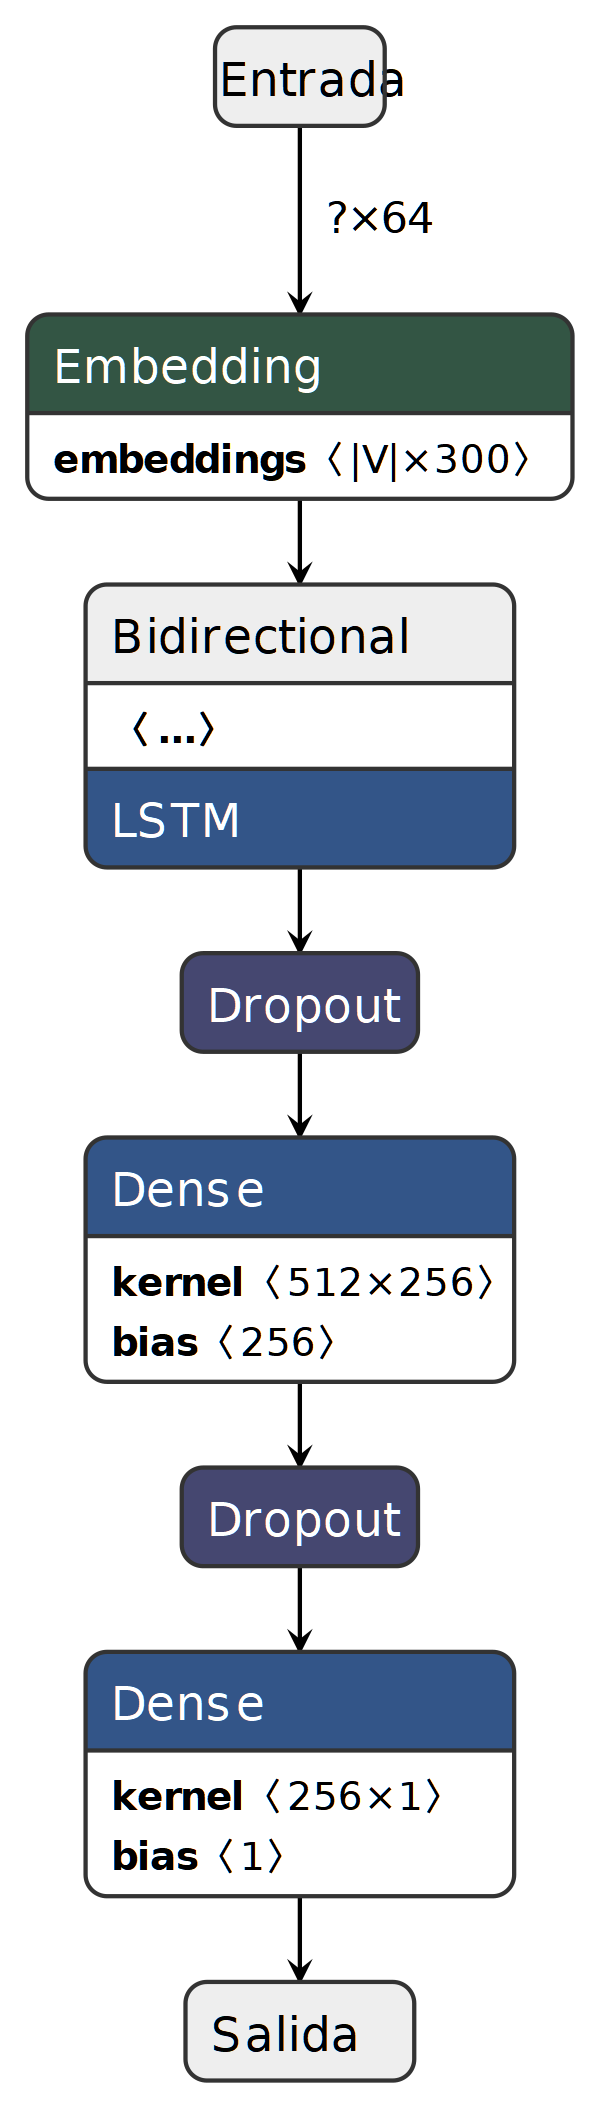
\includegraphics[scale=0.25]{sections/figures/lstm_model.png}
    \caption{Arquitectura del modelo Bi-LSTM}
    \label{fig:lstm_model}
\end{figure}

%%Elminar 

En la figura \ref{fig:cnn_model}, se presenta la arquitectura empleada para la red convolucional (CNN), esta arquitectura esta basada en el trabajo de \citep{kim2014convolutional}. Se implementan tres tamaños de filtro [3,4,5], cada uno con 300 filtros. Los filtros hacen convoluciones en una matriz que representa a la secuencia de palabras y generan mapas de características de longitud variable; la operación de \textit{Max Pooling }se realiza sobre cada mapa, es decir, se calcula el número mayor de cada mapa de características. A partir de esto se obtienen diferentes vectores de características de diferentes tamaños y la penúltima capa se forma concatenándolos, para formar un vector final de características, la capa final recibe este vector de características, para clasificar la secuencia de palabras. Los nodos intermedios de las capas ocultas se activan con la función de activación Relu \ref{eq:RELU}. 

\begin{figure}[!h]
    \centering
  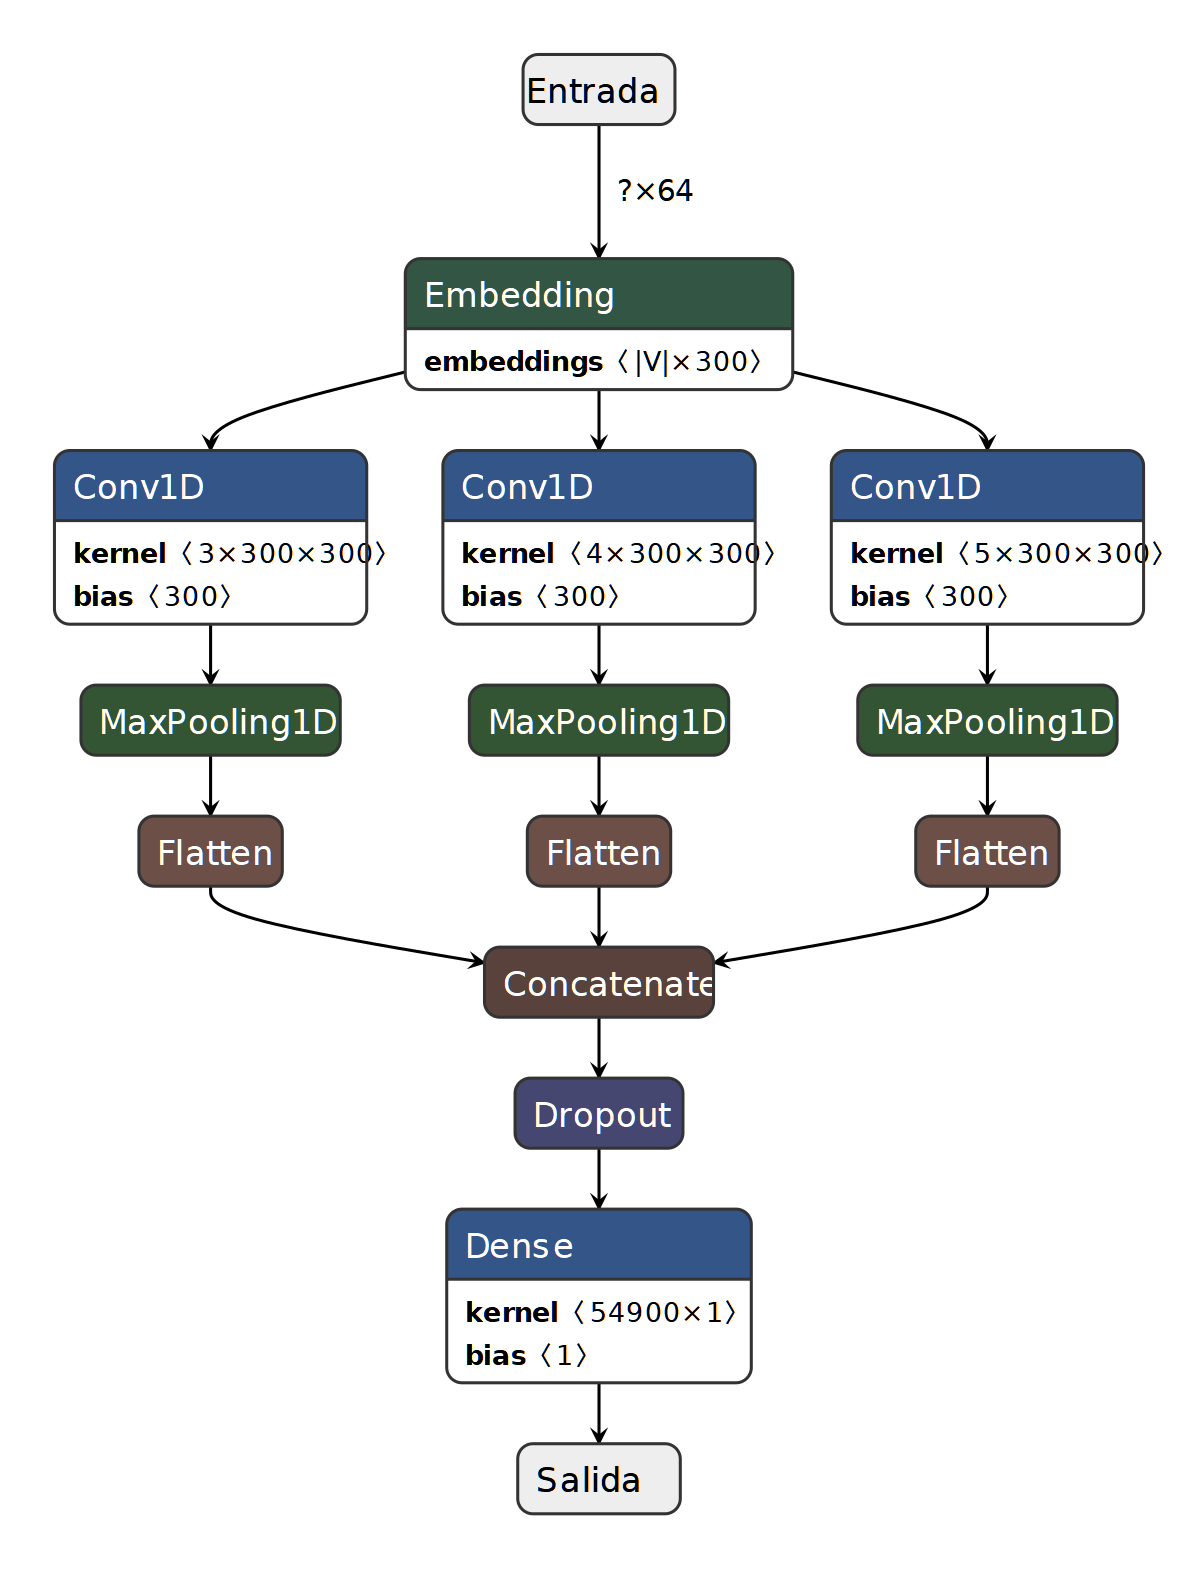
\includegraphics[scale=0.3]{sections/figures/cnn_model.png}
    \caption{Arquitectura del modelo CNN con múltiples tamaños de convolución}
    \label{fig:cnn_model}
\end{figure}


\subsubsection{Entrenamiento}
Para encontrar los hiperparámetros de los modelos se realizó una división del conjunto de entrenamiento en 3 particiones diferentes (3 K-Folds) con una proporción de 66\% para entrenar y 33\% para evaluar.


Observando el desbalance existente en los conjuntos de entrenamiento, por ejemplo, para el conjunto \textit{Depresión 2019}. Se necesita aumentar más de 20 veces la clase positiva para llegar a balancear los datos, por lo tanto, para realizar experimentos consistentes, en caso de los modelos de redes neuronales, se entrenan de forma que sean sensibles al desbalance \citep{wang2016training}, utilizando un peso adicional para cada clase, calculado mediante la fórmula \ref{eq:weights_balance}. Con esto el error es incrementado para ejemplos en la clase de interés y decrementado para la clase menos importante. Esto se realiza para compensar el desbalance que no se alcanza a cubrir con el aumento de datos para cada configuración de $n$.

Los parámetros elegidos para el entrenamiento se resumen en la tabla \ref{table:param_redes}. 

\subsubsection{Evaluación}

Como resultado del entrenamiento se tiene un clasificador. Este clasificador es evaluado a través de un conjunto de datos previamente seleccionado, el cual no ha sido utilizado en la fase de entrenamiento. Cabe recordar que este clasificador, se ha entrenado para determinar la clase de un fragmento del historial de un usuario. De esta forma, la predicción final se realiza observando la clase de todos los fragmentos del usuario en evaluación. Si el número de fragmentos pertenecientes a la clase de interés supera cierto umbral, se considera que se tiene suficiente evidencia para determinar que el usuario pertenece a la clase de interés (véase la figura \ref{fig:metodologia}). En este caso se calculó un promedio de las predicciones pertenecientes a un historial. El umbral de decisión se fijó en 0.5 para los modelos basados en SVM, SVM-C, Bi-LSTM y en 0.4 para la red convolucional CNN. 


\begin{table}[t]
\caption{Parámetros utilizados para el entrenamiento de los modelos basados en redes neuronales.} \label{table:param_redes}
\begin{center}

\begin{tabular}{lc}
\hline
\rowcolor[HTML]{C0C0C0} 
\textbf{Parámetro}      & \textbf{Valor}           \\ \hline
Tasa de aprendizaje     & 1.00E-03                 \\ \hline
Tamaño del Batch        & 1024                     \\ \hline
Función de pérdida      & Entropia cruzada binaria \\ \hline
Máximo número de epocas & 20                       \\ \hline
Criterio de paro    & CNN=6; Bi-LSTM=3         \\ \hline
Pruebas independientes  & 3                        \\ \hline
\end{tabular}

\end{center}
\end{table}

\subsubsection{Implementación}
Para el preprocesamiento y el etiquetado de las secuencias de texto se utilizó la librería NLTK \citep{loper2002nltk}, para la normalización y el cálculo de medidas de similitud de los embeddings la librería gemsin\footnote{www.radimrehurek.com/gensim}.
Los modelos lineales fueron implementados utilizando la librería sckit-learn 0.22.1 \footnote{www.scikit-learn.org/stable/} , los modelos neuronales mediante tensorflow 2.2 \footnote{www.tensorflow.org}. %\citep{tensorflow2015whitepaper}
Finalmente, el 50\% de los modelos fueron entrenados con una computadora personal y el 50\% en Colab\footnote{colab.research.google.com} (una herramienta de acceso gratuito para entrenar redes neuronales en la nube).
